Von einem verrauschten, sinusähnlichen Signal bekannter Frequenz $\omega$
ist die genaue Phasenlage zu bestimmen.
Wegen des Rauschens sind charakteristische Punkte des Graphen des Signals
wie etwa der Nulldurchgang keine zuverlässigen Indikatoren für die Phase
(Abbildung~\ref{60000022:figure}).

Das Signal kann in der Form $f(t) = A\sin(\omega t + \delta)$ geschrieben
werden, der Winkel $\delta$ ist zu bestimmen.
Mit Hilfe des Additionstheorems für die Sinus-Funktion folgt
\[
f(t) = A\cos(\omega t)\sin(\delta) + A \sin(\omega t)\cos(\delta)
=
a\cos(\omega t) + b \sin(\omega t),
\]
wobei
\[
a = A\sin(\delta)
\qquad\text{und}\qquad
b = A\cos(\delta)
\]
gilt.
Insbesondere kann man $\delta$ bestimmen, sobald $a$ und $b$ bestimmt
worden sind.
Gegeben sind 24 Messwerte $f_0,\dots,f_{23}$ des Signals zu 24 gleichmässig
über zwei Perioden des Signals verteilten Zeitpunkten $t_0,\dots,t_{23}$.
Stellen Sie ein Gleichungssystem auf, mit dem sich die bestmöglichen Werte
für $a$ und $b$ bestimmen lassen.

\begin{figure}[h]
\centering
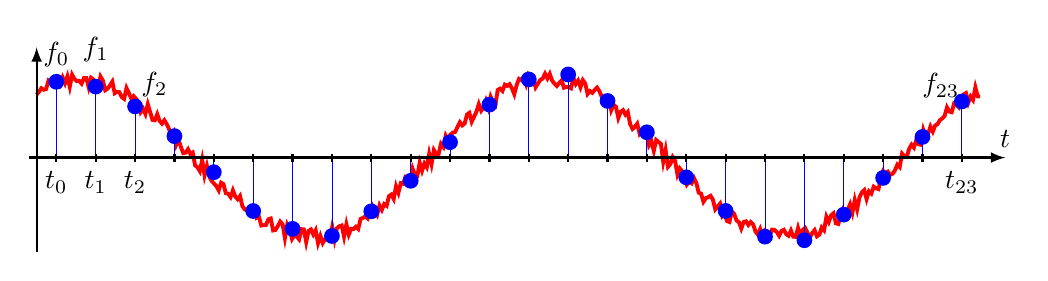
\begin{tikzpicture}[thick,>=latex]
\draw[color=red,line width=1.4pt]
	plot[domain=0:1,samples=400] ({12*\x},{sin(720*\x+60)+0.2*(random()-0.5)});
\foreach \i in{0,...,23}{
	\draw[color=blue,line width=0.3pt]
		({(\i+0.5)/2},0)--({(\i+0.5)/2},{sin(720*((\i+0.5)/24)+60)});
	\fill[color=blue]
		({(\i+0.5)/2},{sin(720*((\i+0.5)/24)+60)+0.2*(random()-0.5)})
			circle[radius=0.1];
	\draw ({(\i+0.5)/2},-0.05)--({(\i+0.5)/2},0.05);
}
\draw[->] (-0.1,0)--(12.3,0) coordinate[label={$t$}];
\draw[->] (0,-1.2)--(0,1.4);

\node at (0.25,-0.05) [below] {$t_0$};
\node at (0.75,-0.05) [below] {$t_1$};
\node at (1.25,-0.05) [below] {$t_2$};
\node at (11.75,-0.05) [below] {$t_{23}$};

\node at (0.25,{sin(720*(0.25/25)+60)+0.1}) [above] {$f_0$};
\node at (0.75,{sin(720*(0.75/25)+60)+0.1}) [above] {$f_1$};
\node at (1.2,{sin(720*(1.25/25)+60)-0.35}) [above right] {$f_2$};
\node at (11.85,{sin(720*(11.75/25)+60)+0.0}) [above left] {$f_{23}$};

\end{tikzpicture}
\caption{Bestimmung der Phase eines verrauschten sinusähnlichen Signals.
\label{60000022:figure}}
\end{figure}

\begin{hinweis}
Eventuelle Matrizenprodukte müssen im Resultat vollständig ausgerechnet
werden.
\end{hinweis}

\thema{Least Squares}

\begin{loesung}
Die Punkte $(t_i,f_i)$ sollten auf dem Graphen der Funktion $f(t)$ liegen,
die Zahlen $\color{red}a$ und $\color{red}b$ müssten daher alle Gleichungen
\[
f_i = {\color{red}a}\cos\omega t_i + {\color{red}b} \sin\omega t_i
\]
erfüllen.
Dies ist ein überbestimmtes Gleichungssystem mit 24 Gleichungen für 
die Unbekannten $\color{red}a$ und $\color{red}b$.
Die Matrix und die rechte Seite dieses Gleichungssystems ist
\[
A
=
\begin{pmatrix}
\cos \omega t_0&\sin\omega t_0\\
\cos \omega t_1&\sin\omega t_1\\
\cos \omega t_2&\sin\omega t_2\\
\vdots         &\vdots        \\
\cos \omega t_{23}&\sin\omega t_{23}
\end{pmatrix}
\qquad
\text{und}
\qquad
b
=
\begin{pmatrix}
f_0\\
f_1\\
f_2\\
\vdots\\
f_{23}
\end{pmatrix}.
\]
Die Zahlen $\color{red}a$ und $\color{red}b$ kann man nun als Lösung
des Gleichungssystems
\[
A^tA{\color{red}x}=A^tb
\qquad\text{mit}\qquad
{\color{red}x}
=
\begin{pmatrix}
\color{red}a\\
\color{red}b
\end{pmatrix}
\]
finden.
Die rechte Seite des Gleichungssystems kann man explizit ausrechnen:
\begin{align*}
A^tb
&=
\begin{pmatrix}
\cos\omega t_0&\cos\omega t_1&\dots&\cos\omega t_{23}\\
\sin\omega t_0&\sin\omega t_1&\dots&\sin\omega t_{23}
\end{pmatrix}
\begin{pmatrix}
f_0\\f_1\\\vdots\\f_{23}
\end{pmatrix}
\\
&=
\begin{pmatrix}
f_0\cos\omega t_0 + f_1\cos\omega t_1+\dots+f_{23}\cos\omega t_{23}\\
f_0\sin\omega t_0 + f_1\sin\omega t_1+\dots+f_{23}\sin\omega t_{23}
\end{pmatrix}
=
\begin{pmatrix}
\displaystyle\sum_{k=0}^{23} f_k\cos\omega t_k\\
\displaystyle\sum_{k=0}^{23} f_k\sin\omega t_k
\end{pmatrix}.
\end{align*}
Die linke Seite ist etwas komplizierter, nämlich
\[
A^tA
=
\begin{pmatrix}
\displaystyle \sum_{k=0}^{23} \cos^2\omega t_k
&
\displaystyle \sum_{k=0}^{23} \cos\omega t_k\sin\omega t_k
\\
\displaystyle \sum_{k=0}^{23} \cos\omega t_k\sin\omega t_k
&
\displaystyle \sum_{k=0}^{23} \sin^2\omega t_k
\end{pmatrix}.
\qedhere
\]
\end{loesung}

\begin{diskussion}
Es stellt sich heraus, dass die Matrix $A^tA$ vollständig berechnen lässt.
Die beiden Diagonalterme sind als Summe von Quadraten natürlich positiv.
Sie sind aber sogar identisch, denn die $\sin$ und $\cos$ Werte
sind nur um $90^\circ$ phasenverschoben.
Mit den Formeln
\begin{align*}
\cos^2\omega t_k
&=
\frac12(1+\cos2\omega t_k)
\\
\sin^2\omega t_k
&=
\frac12(1-\cos 2\omega t_k)
\cos\omega t_k \sin\omega t_k
&=
\frac12\sin2\omega t_k
-
\frac12\sin 0
=
\frac12\sin2\omega t_k
\end{align*}
kann man die Summen explizit berechnen.
Da die $t_k$ gleichmässig über eine Periode verteilt sind, folgt
\[
\sum_{k=0}^23 \cos\omega t_k = 0
\qquad\text{und}\qquad
\sum_{k=0}^23 \sin\omega t_k = 0.
\]
Es folgt daher
\begin{align*}
\sum_{k=0}^{23}
\cos^2\omega t_k
=
12 + \sum_{k=0}^{23}\cos2\omega t_k = 12
\\
\sum_{k=0}^{23}
\sin^2\omega t_k
=
12 - \sum_{k=0}^{23}\cos2\omega t_k = 12
\\
\sum_{k=0}^{23}
\sin\omega t_k\cos\omega t_k
&=
\frac12\sum_{k=0}^{23} \sin 2\omega t_k
= 0.
\end{align*}
Die Matrix $A^tA$ ist also die Diaogonalmatrix $A^tA=12E$.
Damit kann man die Lösungen für ${\color{red}a}$ und ${\color{red}b}$
sofort angeben:
\begin{align*}
{\color{red}a}
&= 
\frac12\sum_{k=0}^{23} f_k \cos\omega t_k
\\
{\color{red}b}
&= 
\frac12\sum_{k=0}^{23} f_k \sin\omega t_k
\end{align*}
Diese Formeln sind natürlich aus der Fourier-Theorie wohlbekannt.
\end{diskussion}

\begin{bewertung}
Lineare Gleichungen für Variablen ${\color{red}a}$ und ${\color{red}b}$
({\bf G}) 1 Punkt,
Matrix $A$ ({\bf A}) 1 Punkt,
Vektor $b$ ({\bf b}) 1 Punkt,
Lösungsverfahren $A^tA{\color{red}x} = A^tb$ ({\bf L}) 1 Punkt,
Produkt $A^tA$ ({\bf P}) 1 Punkt,
rechte Seite $A^tb$ ({\bf R} 1 Punkt.
\end{bewertung}




